\documentclass[11pt]{article}
\usepackage[T1]{fontenc}
\usepackage[margin=1.0in]{geometry}
\usepackage{soul}
%\usepackage[small,compact]{titlesec} %very powerful
\usepackage{tcolorbox}
\usepackage{enumitem}
\usepackage{epigraph}

\usepackage{cite}
\usepackage{caption}
\captionsetup{font=small}
\usepackage{graphicx}
\usepackage{amsmath}
\usepackage{amssymb}
\usepackage{amsthm}
\usepackage{hyperref}
\usepackage{wrapfig}
\usepackage{xcolor}
\usepackage{hyperref}
\hypersetup{
    colorlinks,
    citecolor=black,
    filecolor=black,
    linkcolor=blue,
    urlcolor=blue,
}
\usepackage{booktabs}

\newtcolorbox{cbox}[1][]
{
left=1pt,right=1pt,top=1pt,bottom=1pt,
colback=gray!10,
boxrule=0.5pt
}

\newenvironment{commentbox}[1][]{
\small
    \begin{cbox}
    \textbf{#1}: 
 }{
   \end{cbox}
}


\def\Section{\S}

\newcommand{\mycomment}[3][\color{blue}]{{#1{{#2}: {#3}}}}
\newcommand{\tvn}[1]{\mycomment{TVN}{#1}}{}
\newcommand{\didi}[1]{\mycomment{Didier}{#1}}{}
\newcommand{\tl}[1]{\mycomment{ThanhLe}{#1}}{}
\newcommand{\red}[1]{{\color{red}{#1}}}
\renewcommand{\figurename}{Fig.}
\renewcommand{\tablename}{Tab.}
\title{\vspace{-1in} Demystifying the Computer Science \\PhD Admission in US Universities\\{\large A guide for Vietnamese and International Students}}
%\date{\today}
\author{\small \href{https://nguyenthanhvuh.github.io}{ThanhVu (Vu) Nguyen} (\href{mailto:tvn@gmu.edu}{tvn@gmu.edu})}

\begin{document}
\maketitle

\begin{abstract}
Having been involved in PhD admissions for many years, I've
realized that many \textbf{international students}, especially those from smaller countries such as \emph{Vietnamese}, lack a clear understanding of
the Computer Science PhD admission process at US universities. This confusion not only
discourages students from applying but also creates the perception that
getting admitted is difficult compared to CS PhD programs in other countries.

So I want to give some details about the PhD Admission process and share my opinions and advice for those who are interested in applying for a \textbf{PhD in Computer Science in the US}.
While this document is written for Vietnamese students interested in Computer Science, it should apply to students in many other countries and other majors.
Moreover, while many examples given are for George Mason University, the writing should generalize to other R1\footnote{An \href{https://en.wikipedia.org/wiki/List_of_research_universities_in_the_United_States}{R1 institution} in the US is a research-intensive university with a high level of research activity across various disciplines.} universities  (though \emph{very} top schools could be very selective, e.g., see the \href{https://da-data.blogspot.com/2015/03/reflecting-on-cs-graduate-admissions.html}{admission process} at CMU).

In addition, this document can help \emph{US faculty and admission committee members} understand more about international students, e.g., questions, concerns, and various cultural differences.  By understanding, appreciating, and even leveraging these information, CS programs in the US can attract larger and stronger application pools from Vietnam and other countries.

I wish you the best of luck. And if you follow these advice,
you will at least have a good chance at GMU (see
\href{https://github.com/dynaroars/dynaroars.github.io/wiki/About-GMU}{why
you want to study at GMU}). Happy school hunting!

This document is available on \href{https://github.com/nguyenthanhvuh/phd-cs-us}{Github}. If you have questions or comments, feel free to create a \href{https://github.com/nguyenthanhvuh/phd-cs-us/issues}{GitHub issue} for discussion.
\end{abstract}

\section{Should You Apply?}
\epigraph{\vspace{-0.2in} Don't make fun of graduate students. They just made a terrible life choice.}{The Simpsons}

First, I want to emphasize that PhD students in Computer
Science \emph{do not} need to worry about funding, especially at good R1
universities in the US. If you are admitted, you will almost certainly
receive \emph{full funding} to support your study, including tuition,
health insurance, and stipend. Moreover, depending on the university,
you may even receive additional benefits such as summer salary, laptops, (conference/workshop) traveling. \S\ref{sec:funding} provides more details on funding.

Second, I believe that applying to a good US university \emph{should not} be any
harder than at schools in other countries. If you think you have a chance in other countries, e.g., South Korea, Singapore, Germany, UK, Japan and Australia, then you will surely have a chance in the US as well.

\begin{commentbox}[Vu]
One of the reasons I create this document is that my (non-Vietnamese) colleagues at GMU are interested in 
recruiting Vietnamese students and are surprised when seeing very few applications in Vietnam (e.g., each year our CS program receives more than 350 PhD applications, most of which are international but only 3--4 are from Vietnam). In general the number of
PhD applications from Vietnam to US universities is few and  more would be very welcomed. 
\end{commentbox}

%% Vu: *what's a PhD?*  This [[https://matt.might.net/articles/phd-school-in-pictures/][series of pictures]] from [[https://matt.might.net][Matt Might]] illustrates what a PhD means.
%% \end{commentbox}


\section{How is Your Application Evaluated?}

After you submit your PhD application (usually in December), it will be first screened
for general requirements, e.g., did you submit your transcripts and standard scores? did your reference writers submit their letters?
Then your application will be reviewed by a
\textbf{PhD admission committee} that consists of faculty members in CS. Each application is assigned to about \emph{three} faculty members, who will evaluate your profile and try to reach a consensus about your case.  Note that while the assigned reviewers are likely the main ones deciding your application, \emph{every} faculty in the department will have access to your application and can give inputs on your profile.

In many cases, the admission committee involves assistant professors in the department. This provides junior faculty the opportunities to recruit students. The chair of the committee will be a senior professor, but they likely will not review individual applications and instead assign them to committee members. The chair will look at various factors such as research interests or mentioning faculty names to assign the applications to appropriate faculty. 

\begin{commentbox}[Vu] 
We usually decide that a PhD candidate is either (i) admit with funding (TA or RA) or (ii) rejected. In other words, in most cases, we either
admit you with full funding, or we don't. In some rare cases, we admit
without funding because you have funding on your own (e.g.,
supported by your government or having external grants). We also justify
our decision with a summary about your application, where we list
strengths (e.g., well-known school) and weaknesses (e.g., weak
LORs). 
\end{commentbox}

%\didi{Is there more information on typical strengths and common weaknesses of applications. This is especially useful to sophomore and junior students as they still have time to work on those strengths.}
% tvn: the main thing is research experiences

\begin{commentbox}[Hakan]
At GMU, for full consideration, students should make sure to submit \textbf{ALL} required documents by the application deadline, and should never assume that some required documents (such as official TOEFL scores or official diplomas/transcripts) will be waived by the admissions office. If something is listed and not marked as "optional", it is mandatory and they should plan for submitting all those.  
\end{commentbox}
\paragraph{Why we do not waive application fee?}  This is typically a requirement of the university. Individual departments/programs do not have the flexibility to waive the application fee, even if they want to. 

In my opinion, requiring applicants to pay the fee helps ensure their seriousness, as it filters out non-serious candidates. Also, if the application process were free for everyone, we would receive an overwhelming number of applications to review.


\section{Application}\label{sec:application}

The primary focus of the admissions committee is to \textbf{evaluate your background and interest in research} since a PhD in Computer Science
is a research degree. To assess your research capability, we consider
the following key indicators, listed in order of importance.

\subsection{Research Ability}

The most effective evidence of research ability is having \textbf{published papers in reputable international journals or conferences}.
Having published good papers is a sign that the applicant has successfully involved in research.

It's important to aim for the top venues in your field, which you can
find on places such as CSRankings~\cite{csrankings}, which ranks CS programs based on how their faculty publish at top \emph{conferences}. Local conferences and non-English journals or conferences do
not carry as much weight since their quality is often unknown to US faculty.


However, I understand that many international students do not have the opportunities to publish in top places, so general confs/journals would suffice.  But be sure to upload your papers with your application and talk about them in your \hyperref[sec:research-statement]{statement}.

\begin{commentbox}[Vu]
Many international students mention Scopus Q1, which consists of various journals from IEEE, Elsevier, and many other publishers.  I don't know/recognize many of journals listed in Scopus Q1 and. This might be something to be mindful of, as \textbf{CS} faculty might not be too familiar with Scopus or journals listed in there, so devote sometime in your statement to discuss the significance of your papers.
\end{commentbox}

\begin{commentbox}[Craig]
GMU and many other universities allow you to upload your published papers and other writing samples. In many cases, even if the papers were not published at top places, we can still determine their quality by simply skimming over the paper.  
\end{commentbox}

Additionally, \textbf{work experiences at renown research laboratories}, such as Microsoft Research, can significantly strengthen your
application.  Unfortunately, many good research places in your countries, e.g., VinAI in Vietnam, remain relatively unknown to most universities in the US. So you should explicit say something about them in your statement.

Finally, \textbf{participating internationally recognized competitions} can also demonstrate your research potential.
For example, participating in Math Olympiads if you want to do theory or  winning ACM programming contests if you want to ``build'' stuff, e.g., software analysis.

\begin{commentbox}[Thanh]
Due to academic culture, professors in Vietnam usually aim for (international) journals instead of conferences. Could you give some tips on how to know whether a journal is good (CSrankings, unfortunately, only consider conferences)?.
\tcblower
Vu: One way is looking at what well-known researchers publish at. For example, if you are interested in a field X, you can use CSRankings to look at active faculty in X, and then look at their websites to see what journals they publish at.
\end{commentbox}

\subsection{Letter of Recommendation (LOR)}\label{sec:lor}

Most CS PhD programs will require at least \textbf{two LORs}. Having a letter from an internationally recognized researcher can greatly strengthen your application. However, obtaining such letters
can be challenging for international students, who might not have much interactions with such experts. So it is acceptable to have a letter from professors that know you well enough to talk about \emph{your specific research experience and capabilities}.

\begin{wrapfigure}{r}{0.47\textwidth}
    \vspace{-0.35in}
      \begin{center}
        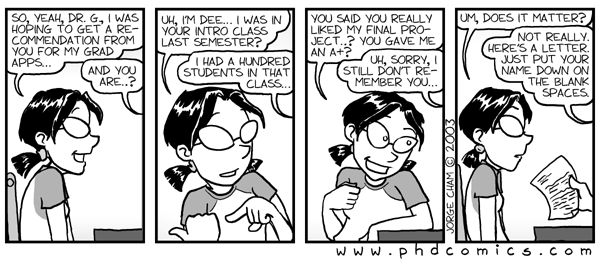
\includegraphics[width=0.47\textwidth]{c6.png}
      \end{center}
    \vspace{-0.4in}
    \end{wrapfigure}
Many students have letters written by the applicants themselves and signed by their professors. These have little
values (we can easily recognize them) and will consider them weakness.
Similarly, many professors write very generic letters for students (a common example is that the students didn't do any
research or make any impression for the professor to write about). These letters are also not useful and considered weak.

Many students get letters from supervisors from company where they did internship or are
working at. It is OK as long as it is a research-based personalized
letter (once again, we are talking about PhD applications, not MS).


\begin{commentbox}[Vu]
Some letter writers ask the applicants to write their own letters for them to sign. As mentioned, this will hurt the applicants (admission committee members are actually quite good at determining this)! I was also told that some people did this so that the applicants do not go abroad or only go to places where they want the students to go to.
\tcblower
Sometimes students would go through great length just to get letters from well-known professors in their school, but the letters are generic and carry little value, in fact, \red{red flags}. Moreover, a top professor in Vietnam might not be well-known to US faculty (see more details in \S\ref{sec:your-school}). So save the trouble and just get letters from \emph{any} professors/supervisors who knows you well and can write a good letter about your research ability. It's better to have a good personalized
letter about your own research ability from someone who is less
well-known than a generic/weak letter from a well-known person.
\end{commentbox}

\begin{commentbox}[Didier]
\emph{Should letter writers have PhDs?}  In Rwanda, a lot of students interact more with teaching faculty who might not have PhD.
\tcblower
\textbf{Vu}: In general, at least one writer should have PhD to properly evaluate your research ability.  However, I think this is an interesting and useful detail that US faculty might not be aware of and students should mention about this in their statements.
\end{commentbox}

\subsection{Research or Personal Statement}\label{sec:research-statement}

While you might not have control over LORs \hyperref[sec:your-school]{where your go to school}, you do over your
statement! So write it well because we do take it seriously.
A well-written LOR also shows that you can communicate, which is very important in research, and that you can effectively teach and communicate with students, which is important for TA funding (see \S\ref{sec:funding}).
%is important because if you need (GTA) funding, it will provide evidence
%that you can teach and communicate with students.

There are various guides on writing statement, e.g.,~\cite{blattman2022writing}, and \href{https://cs-sop.org/}{many example statements} are available. So I will not talk too much about statements. In short, discuss about your research vision and convince us that you can achieve it through your experience, e.g., published papers, or if you work on some projects by yourself, talk about it. Also, use the statement to talk about stuff that admission committee members might not know about, e.g., your Github project with 1K+ stars or  your regular contributions to well-known open-source projects.

\begin{wrapfigure}{r}{0.50\textwidth}
\vspace{-0.4in}
  \begin{center}
    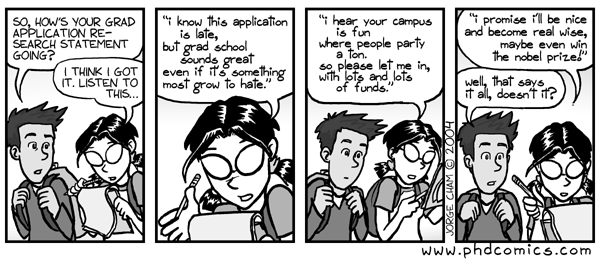
\includegraphics[width=0.50\textwidth]{c2.png}
  \end{center}
\vspace{-0.4in}  
\end{wrapfigure}
Finally, this is something easy to do, but is missed by many
applicants: \textbf{customize the statement} for the school you're applying to,
e.g., why do you apply here? talk about a couple of professors who you're interested in working with (in many cases your application will be forwarded to them for evaluation).
This shows that you're serious and have done homework on places you're applying to.
Be careful not to send statements to wrong schools or mixing
facts (e.g., talking about school X but mentioned about working with
profs. at school Y; and definitely do not talk about George Washington when applying to George Mason). I have seen such statements more time that I
should.


\begin{commentbox}[Vu]
I always read the research statement first and then LORs. If I am
persuaded by then, I would skim over other factors and advocate for
admission (unless I see red flags in other parts). If I am not
convinced, then I will likely recommend rejection (unless I see
something standout in other parts).
\end{commentbox}


\subsection{Your School}\label{sec:your-school}

Graduating from top universities \emph{that we recognize} helps.
However, if committee members do not know much about schools in your country, they will likely treat your school as
\emph{``unknown foreign''}, which can be a minus point (if your school is well-known, then it is \emph{``top foreign''}, which is definitely a plus).

So what can you do about this? several things such as asking your CS dept to put itself on CSRankings (it's the easiest way to get CS people to know about the school), explaining about your school in your statement (and asking your LOR writer to do that too), and of course, if you're interested in working with Vietnamese professors, consider a PhD program in the US that  \href{https://github.com/dynaroars/dynaroars.github.io/wiki/Viet-CS-Profs-US}{have them}.

\begin{commentbox}[Vu]
Sometime PhD admission committee will share a document such as \href{https://github.com/dynaroars/dynaroars.github.io/wiki/Foreign-Top-Schools}{this one}, which lists the top schools in several countries. Personally I have looked at Vietnamese applications (whether they are assigned to me or not) and provide input to their reviewers, e.g., X is the top tech school in Vietnam and so it should be \emph{top} instead of \emph{unknown} foreign, which makes a huge difference.
\end{commentbox}

\subsection{Grades/GREs}\label{sec:grades}


Having good grades is important, but unless your school is well-known, having top grades/ranks
usually will not help. This is simply because we cannot evaluate them.

This can be an issue for students in many top international universities where the competition is so high that very good students students can still have low ranking (and be overlooked by Admission committee).
So what to do with this? well, same as \hyperref[sec:your-school]{before}, e.g., put a note about this in your statement and ask your LoR writers to talk about it.

Note that while having good grades at unknown school might not help,
having very bad grades will be \red{red flag} (unless your LORs or
statements give proper explanation). This is especially true if you
have bad grades in relevant, e.g., CS and Math, courses.

\begin{commentbox}[Thanh]
Vietnamese universities typically offer specialized programs, such as the talented engineer program at HUST, that have highly competitive entrance exams and a limited number of available slots (e.g., 30 per year). However, these programs often set higher requirements for students, including more demanding tests and assignments, resulting in lower GPAs and overall rankings. For example, an 3.5 GPA students from such talented programs are typically much better than a 4.0 GPA students not in those programs.  Similarly, variations in GPA standards exist among different universities, with technical universities generally having lower GPAs than economical universities. These make gaining admission in the US difficult as US faculty are not familiar with these issues.
\tcblower
\textbf{Vu}: Many Vietnamese students and faculty lament how this competitive/low-grading from top Vietnamese universities hurts its own students in applying abroad. One way to mitigate this is making these issues known to admission committee.  Schools with Vietnamese profs are probably aware of them, but in general your letter writers/you can explicitly mention these in their letters/ your statement.
\end{commentbox}

\paragraph{GRE} Most CS programs in the US \emph{no longer require GREs}, so you don't need to
take them. However, they might be useful for international students from programs we are not familiar with. 

\paragraph{English Test} Unless your degrees are from certain countries such as \href{https://github.com/dynaroars/dynaroars.github.io/wiki/About-GMU#standard-tests-waiver-eligible-countries}{these}, you will need to
take standardized English test. Just do well enough to pass minimum requirement set by the university, which nowadays has many options for you to choose from.

\begin{commentbox}[Vu]
The minimum for GMU (being above this might not mean much, but below is a \red{red flag}).
\begin{itemize}
\item GPA: $\ge 3.0$ in your undergrad (but we also consider the rank/prestige of your school)
\item GRE: not required, though it can help boost your profile
%    \item but if you want to use it, then we expect a total (V+Q) of $\ge 311$ (with a $\ge 157$ Q) and A $\ge 3.0-3.5$.
\item English requirement tests (one of the below)
  \begin{itemize}    
  \item TOEF: 88 pts in total AND $\ge 20$ points in each subsection OR
  \item IELTS: $\ge 6.5$ OR
  \item DuoLingo Graduate English: $\ge 120$ OR 
  \item Pearson Test of Academic English: $\ge 67$
  \end{itemize}  
\end{itemize}
\end{commentbox}


\subsection{CV/Resume}
This should be a summary of the accomplishments of the applicant.  It should allow the reviewers to quickly scan to identify standout achievements (e.g., Publications, Programming Competition Awards, Teaching Experience).

\subsection{Interview}

Sometime a faculty wants to interview an applicant to make a decision. This means they are leaning toward admitting you (if we don't like your application, we will not bother doing the interview).

An interview lasts about 15--30 mins, and one implicit thing you will be evaluated on is whether you can communicate effectively (i.e., speak/understand English).  You will also get chance to ask questions about the university so think of something to ask (just the same as you interview at a company).

\begin{commentbox}[Vu]
At GMU, we are encouraged to interview candidates. For very strong candidates, the interview is actually to recruit them.  In some cases a faculty interviews a candidate that they see potentials and wants argue for admission, i.e., without the interview, that candidate is definitely rejected. In any case, getting interview means you have a very good chance of being admitted.
\end{commentbox}

\section{Getting Admitted and Choosing the Right School}

Around March you should hear back from most PhD programs that you applied to (if not, send email and ask).
If you have offers, congratulations!  Now you're at a different game because the schools that admit you will now try to get you to accept them!   You will likely have to make your decision by around April 15.

Most schools will have an \textbf{Open House}, which is a great resource to learn about the school, department, faculty, research, living, etc. During the Open House, you get a chance to talk to individual faculty and current students.  Take notes of faculty who make you excited, count those that are taking in new students (if they meet you, likely they are considering new students!).  Talk to students about their advisors, the dept, the area, funding situation etc.  Ask about anything you want to determine that they deserve \emph{you}.

In short, if you can come to the Open House, do come.  But if you're international student outside of the US, then likely you cannot come.  So see if you can attend it virtually and meet with individual faculty.

\begin{commentbox}[Vu]
GMU has \emph{Virtual} Open House (VOH), e.g., \url{https://cs-gmu.github.io/cs-phd-voh-s23/}, which I've co-organized in the last two years. We invite all admitted PhD students to the VOH through Zoom to learn about the CS program, the department, GMU, and the DC area in general. Students also get opportunities to chat with professors and current students.
\end{commentbox}



\section{Funding}\label{sec:funding}

As mentioned, if you're admitted to a \emph{good} CS PhD program, you should not have to worry about funding!  
In the US, the common types of funding for PhD are \emph{graduate teaching assistant} (GTA or TA), \emph{graduate research assistant} (GRA or RA), and \emph{Fellowship}.
RA is paid by a prof. for you to do their research. TA is paid by the department for you to help with teaching. Finally, fellowship is an independent funding that come from a school, a company, or an organization. Tab.~\ref{tab:funding} summarizes the differences.


Note that funding is typically more available for PhD students than 
Masters and especially undergraduate studies, which typically have no funding (and they also have to pay international tuition, which is very expensive!).  

\begin{table}
  \centering
  \footnotesize
  \caption{Different types of PhD funding}\label{tab:funding}
  \begin{tabular}{c|c|c|c}
    \toprule
    &\textbf{TA}&\textbf{RA}&\textbf{Fellowship}\\
    \midrule
    \textbf{From} & School & Profs. & School/External\\
    \textbf{For}                  & Teaching Assistant       & Research                        & Research                              \\
    \textbf{Tuition/Ins./Stipend} & Yes                      & Yes                             & Yes                                   \\
    \textbf{Cover Summer?}              & No                       & Maybe                           & Yes                                   \\
    \midrule
    \textbf{Pros}                 & Research Freedom         & Get to do research              & Research Freedom                      \\
    \textbf{Cons}                 & TA, Uncertain            & Research restriction, Uncertain & Competitive, limited             \\
    \bottomrule
  \end{tabular}
\end{table}

\subsection{Graduating Assistantship (TA/RA)}
The most common type of funding is \textbf{graduate assistanship}, which is either TA or RA. Both TA and RA come with tuition waiving (you don't have to pay tuition), health insurance (this takes care of your insurance, which is a must have in the US), and most importantly, your stipend (i.e., your salary). Some universities also pay insurance for spouse/children (or give very good discount).

Several words about stipend. First, the amount of stipend depends on the university, which in turns depend on various factors such as location (e.g., a stipend in Washington DC is likely higher than in Lincoln, Nebraska due to higher living cost). Second, a school year is (typically) 9-month in the US, so stipend is for 9 months (so divide by 9 for each month). Third, like for most source of income in the US, you will have to pay tax on your stipend. Finally, private universities might pay more for stipend.

\begin{commentbox}[Vu]
TA and RA at GMU have similar benefits in tuition waiving and insurance.  For stipend, the college and department will set a 9-month graduate assistant stipend.  TA and RA will usually be that amount (TA will likely be that amount but RA might be higher depending on the stage of the student (1st year vs ABD\footnote{All but dissertation: really close to graduate.}) and the prof.). 
\tcblower
Having health insurance is required at many US universities.  So do not think that you're young and healthy and ignore insurance.  At GMU, and at most good CS PhD programs, your GTA or GRA \emph{will always} come with full insurance. In fact, at GMU your spouse/children will get significant discount rate for health insurance.  So you will never have to worry much about health issues for you or your family here.
\end{commentbox}


\subsubsection{Teaching Assistant (TA)}

TA is common in the beginning when you haven't found your advisor who would pay you RA. As a TA, you spend up to 20 hrs/week and help professors with their classes (e.g., grading or teaching labs/recitation). Your TA is paid through the school/department, i.e., they hire you to help teach.  During a semester, a TA might work with several courses and professors (not necessary their advisor).  TA funding typically is not available during the summer, which has no school.

\paragraph{How to get TA?}  Unless you have other funding such as RA or Fellowships, TA is typically a default thing. When you apply to be a full-time student,  state that you need financial assistant. It is common that the PhD committee will either admit you and give you GTA, or reject you; i.e., we do not admit a student without supporting them.  

\begin{commentbox}[Vu]
At GMU CS, students admitted with TA have  4 years of GTA guaranteed and also receive  stipend for the \textbf{first} summer.
\end{commentbox}

Even if you have other funding and do not need TA, you still should do TA at least once.  This allows you to see what teaching is like, which is especially helpful for research career where you often give talks and tell people about your work. Note that GMU sometimes has classes that a more senior student can teach.  In that case, you will be paid as a lecturer, which is higher than GTA.  This is a good opportunity for students to get teaching experience and also get paid more.
\subsection{Research Assistant (RA)}
RA is provided through a professor through their own funding so you can work on their project.  
You do not need to teach as an RA, so you can focus on your research. Depending on the professor, RA may be available during the summer. \S\ref{sec:ra-cost} gives more details on RA budget.

\textbf{How to get RA?} When a professor recruits you, they will likely give you RA right away (e.g., when you apply).  A common scenario is that you first get admitted with TA, and then after a year or two find an advisor to support you with RA. 


\begin{commentbox}[Vu]
If you got recruited by a prof. who would give you RA right away, it's very likely you will get admitted.  For example, if a prof., even if not in PhD admission committee, wants to work with and funds you, the PhD admission committee will respect that decision and admit your application (unless your application has many red flags).
\end{commentbox}

\subsection{Fellowship/Scholarship}

Fellowship is another type of funding that the student needs to apply for (e.g., from school, industries, government). Fellowships are typically competitive and generous, and gives pretty much all benefits tuition/insurance that a TA/RA has.  Moreover, it often gives higher stipend (including summer) and opens doors for job opportunities (e.g., internship).  For example, a student with a Microsoft fellowship will likely get an internship at Microsoft.  

In general, fellowship is prestigious, and you will stand out if you get one.  Every PhD student has pubs, but only superstars have NSF grad or Microsoft fellowship. In fact, these are so prestigious that even if you didn't get it but make it to the final round, school will still mention you on their website and you still should put it on your CV.


\textbf{How to get Fellowship?} You apply for them.  The US government has many fellowships that would likely require US citizenship or residency.  However, tech companies including Google, Microsoft, Facebook, IBM have fellowships that international students can apply for. 

Prestigious fellowships typically require a clear and good research plan, so it is a good idea to wait until at least your second year to have research experience and even publication before applying. Remember, you're competing with the top PhD students at top universities worldwide. 


\begin{commentbox}[Vu]
At GMU, PhD applicants are automatically eligible for a Presidential Fellowship.  It is at least as good as GTA but the most important thing is that as a fellowship it is truly free money (i.e., you are not depending on any prof. or TA duties).  PhD admission committee members nominate applicants for this fellowship and the committee will vote and give the fellowship to the top 2.
\end{commentbox}


\section{Miscs and FAQs}

\subsection{What can you do to increase your admission chance?}

 Show something that makes you \textbf{stand out}, e.g., are you a female or a minority in CS (research for this on Google)? Do you participate in outreach activities that help increase diversity and inclusion in CS?  All of these are important in CS in the US.
    
Even if you do not have research experience, you can talk about your personal projects. For example, if you have an open-source project on Github that is used by many people, has lots of stars in Github, do talk about it. If you write technical, research-like blogs, talk about them too.

\subsection{How to rank or select a CS program?}
   \begin{center}
    
\includegraphics[scale=0.4]{c1.png}
   \end{center}

International students not familiar with US universities often put them into \emph{two} bins:  (i) very top school that they dream about such as Stanford, MIT, Princeton, Harvard and (ii) everything else.  Sometimes they rank CS programs using the reputations non-CS programs, e.g., medical or physics.
In some cases they rank universities based on popular states they know in the US, e.g., California and New York.  Let's just say there are so many thing wrong with these methods.

You can learn about CS programs and research expertise of faculty using resources such as \href{https://csrankings.org}{CSRankings.org}, which is designed specifically to help prospective PhD students in Computer Science!  You will be very surprised to learn that a school X that you didn't know much about has very strong research in your interested field Y. This is also a good way to learn about individual faculty (who works on what) and well-known CS conferences\footnote{In CS (and only in CS), conferences, not journals, are often the main venue to publish research finding.}. \S\ref{sec:ranking} gives the top 50 CS programs in the US according to CSRankings.
\begin{commentbox}[Dat] Most Vietnamese students, including those from top schools, do not know about CSRankings.  May be applicants who worked at top research places such as VinAI would know about it.
\end{commentbox}

More generally, rankings can be superficial and you need to do more research to be informed and make better decision. For example, if you get admissions to several places, you should contact profs. that you're interested in at those place and talk to them. They would be more willing to chat to you now that you have been admitted.  Ask them questions about their work, how they manage students, their expectations. You can even ask to contact their students.


\subsection{Tenured or tenure-track faculty? Who do you choose?}

\begin{wrapfigure}{r}{0.48\textwidth}
    \vspace{-0.3in}
      \begin{center}
        
\includegraphics[width=0.48\textwidth]{c8.png}
      \end{center}
    \vspace{-0.2in}
    \end{wrapfigure}
The short answer is that tenured-track faculty (e.g., assistant professors) are more likely to be young and active in research (they have to, in order to get tenure). Thus, they will likely have more time to work with you and push you to do research and publish. However, they may not have as much experience in managing students and may not have as much funding as tenured faculty.
Tenured faculty (e.g., associate and full profs.) are more likely to be older, more well-known, and have more experience in managing students.  However, they might not push you as hard (they don't have to, they already got tenured) and expect you to figure things out yourself (so you need to be very independent).  Some tenured faculty are also no longer active in research, e.g., they are more involved in administrative duties. 

You can learn about faculty and their level of research activity through the faculty's website and CSRankings.
Ultimately, choose one that fits you the most by communicating with them, meeting them, asking them questions, even talking to their students. 


% \subsubsection{Strong Faculty vs High-ranked School}
% \begin{commentbox}[Thanh]
% When considering PhD programs, we often wonder if we should prioritize a high-ranking university or a professor with a strong reputation? Of course, both are great, but it is hard to achieve both.  I believe receiving some guidance from you  would be incredibly valuable.
% \end{commentbox}

% This is a good question and there doesn't seem to be any best answer or specific algorithm that you can use.  But I'll throw out something for you to think about. To me, there are many good schools in the US and so you have some leeway in choosing.  For example, I don't believe there's much difference among schools in top 5 (e.g., CMU, UIUC, UCSD, MIT, GTech are in the same equivalent class), top 10 (e.g., Michigan,  Stanford, UWash, UC-Berkeley, Cornell is another equivalent class), top 20, top 30, top 40, and so on (though I would say schools above 100 are pretty much in the same equivalent class).  It's hard to say a top X is much much better than a top X+20 (e.g.,  Purdue at 15 is stronger than Yale at 35, but not \emph{that much} stronger as you would think).  So keep that in mind, while ranking does matter (e.g., more active faculty, stronger students), the lower ranked universities are still pretty good, might have sub fields that are extremely strong (NCState is 40th, but in Software Engineering it is easily top 5), and many unique things.  This is in contrast with universities in Vietnam where there are large gaps among the top 5, 10, and so on.  




\subsection{Can I apply to CS PhD if my undergrad was not in CS or related areas?}

Yes, as long as you can demonstrate you are ready for CS PhD research through research experiences, LoRs, statements, etc as mentioned. You might be even able to leverage this to make your profile stand out.



\subsection{Is an MS degree required for admission to PhD?}
No. In fact, student with BS can get MS degree "along the way" to PhD.  However, MS can help if it gives research experience or is from a more well-known school than your undergrad institution.
    

\subsection{How long does it take to complete the PhD program?}

\begin{wrapfigure}{r}{0.28\textwidth}
    \vspace{-0.4in}
      \begin{center}
        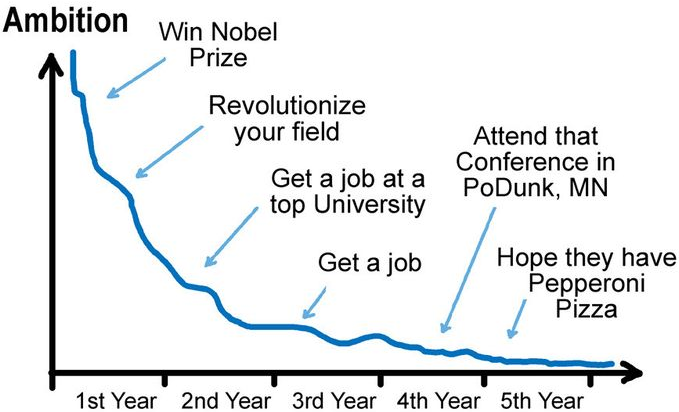
\includegraphics[width=0.28\textwidth]{c4a.png}
      \end{center}
    \vspace{-0.2in}
    \end{wrapfigure}
    Typically, 5-7 years for PhD in CS at US universities.  The first 1.5--2 years you spend on coursework and learning research.  The next 2--3 years you focus on your research, formi dissertation topic, and get results published.  The last 1-2 years you write and defend your dissertation and look for job. The PhDComics figure on the right shows the "ambition" level of a PhD student over their years of study (they miss the 6-7th Year where the ambition is "Please just get me graduate").



\subsection{How do I address a professor?}

\begin{wrapfigure}{l}{0.5\textwidth}
    \vspace{-0.4in}
      \begin{center}
        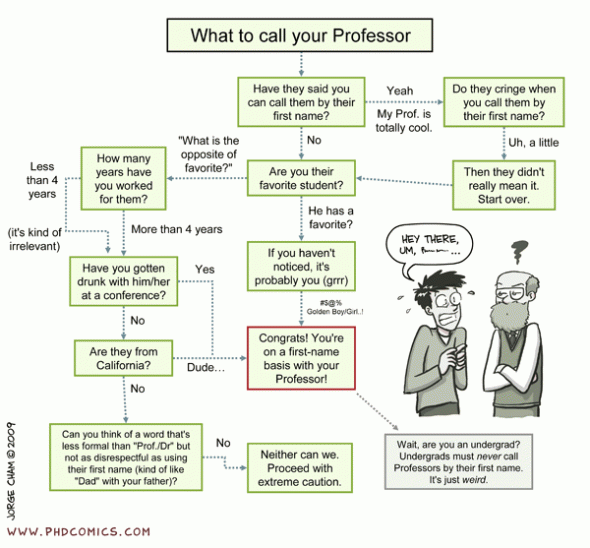
\includegraphics[width=0.5\textwidth]{c5.png}
      \end{center}
    \vspace{-0.9in}
    \end{wrapfigure}
If you don't know the professor (e.g., first email contact), then use \textbf{Prof. Lastname} or \textbf{Dr. Lastname}. I've seen many international students write \textbf{Prof.} or \textbf{Dr.} \textbf{Firstname Lastname}.  Writing like that makes it like you copy and paste the names, so no need to do so,  just Prof. or Dr. Lastname.
        
If you don't know the prof., do not use Mr. or Mrs., or Firstname. To me it seems a bit disrespectful. As you know that prof. better and depends on their preference, you can call them by their Firstname.


\begin{commentbox}[Vu]
    I've been called Dr. Vu and I find it a bit amusing but am totally fine with it.
\end{commentbox}

\subsection{How much do \emph{you} cost?}\label{sec:ra-cost}
PhD students often wonder why their salary is so low compared to ludicrous grants their advisors get or why their offer letters sometime mentioned that their benefits worth way more than what they actually receive (i.e., stipend).  This section aims to shed some light to these questions.

Tab.~\ref{tab:cost} shows the budget breakdown for a GRA per year (this level of details is what faculty actually uses when applying for funding).
These numbers are based on my experience at public universities in the US.  Private universities may have different numbers.  For simplicity, I will assume the department has a 9-month stipend of \$27000 (GMU actually pays more) and therefore a 3-month summer of \$9000. I will also use GMU tuition rate of about \$15,000/year for full-time study (which is quite cheap compared to private universities, e.g., MIT charges around \$50K) and a 58.9\% (overhead) rate on \emph{indirect cost}, which is what GMU charges for administrative costs (yes, after all, universities are businesses!).  Finally, I assume the student makes conference trips per year, one domestic and one international (so conf. registration, airline tickets, taxi, meals, etc are all included). At the end, the total budget comes out to be \$69K.  \emph{The summary is that while you're paid X, your advisor probably pays 2X for you}.

\begin{table}
    \centering
    \small
    \caption{GRA cost breakdown. F \& A is Facilities \& Administrative Cost Base and 
    MTDC is Modified Total Direct Cost. These are things that the university can charge overhead to.}\label{tab:cost}
    \begin{tabular}{rcl}
        \textbf{Budget} & \textbf{Cost \$} & \textbf{Notes} \\
        \midrule
        GRA (9-month) & 27K & \\
        GRA (summer)  &9K	& 3-month, 20hrs/week\\
        \textbf{Total Salary} &\red{36K}	&\\
        \midrule
        Health Insurance	&3K	& full year\\
        Tuition (In-State) &	15K	& (\$680/ Credit + \$150/Student Fee/ Credit)* 9 credits = \\
        &&\$7470 (\$6120 + \$1350) per semester\\
        \textbf{Total Tuition \& Insurance}	&\red{18K}	&Full year tuition + insurance\\
        \midrule
        Conference Registration	& 500 & \\
        International Travel &	1800& \\
        Domestic Travel	& 700	& \\
        \textbf{Total Travel}&	\red{3K}	\\
        \midrule
     Total Direct Cost	& \red{57K}	&Salary + Travel + Health + Tuition \\
     F \& A (MTDC)	& 21K	& Direct Cost - GRA Salary\\
    Total Indirect Cost	& \red{12K}	&58.9\% of MTDC\\
    \textbf{Total (Direct + Indirect)} &	\red{69K}	& Budget for a GRA\\
        \bottomrule
    \end{tabular}
\end{table}

%\subsection{Having fun during a PhD?}
%PhD students \emph{and faculty} probably find it amusing about the notion that students, especially international ones, can genuinely enjoy their PhD studies. In fact, after reading posts after posts on VietPhD.org on how PhD students are commonly mistreated, stressed, it seems being miserable is a norm during a PhD study.

%There are many advice on surviving PhD that you can follow. But here I just list a few that works for me and what I advice my students to do.\tvn{TODO}


\section{Ranking of CS PhD programs in the U.S}\label{sec:ranking}
  Tab.~\ref{tab:ranking} lists the top 50 CS programs in the US from \href{https://www.csrankings.org}{CSRankings.org}, a ranking system  based on top CS conferences.
  
  \begin{table}
    \centering
    \small
    \caption{Top 50 CS PhD programs in the U.S. (CSRankings, June 2023). \red{$^*$} indicates that the university has \href{https://github.com/dynaroars/dynaroars.github.io/wiki/Viet-CS-Profs-US}{Vietnamese prof.} that can advise CS PhD students.}\label{tab:ranking}
  \begin{tabular}{rl|rl}
    \toprule
    1 & Carnegie Mellon & 26 & Univ. of California - Irvine \\
    2 & Univ. of Illinois at Urbana-Champaign\red{$^*$}  & 27 &  Duke University \\
    3 & Univ. of California-San Diego & 28 & Rutgers University\red{$^*$} \\
    4 & MIT & 29 & Univ. of California - Riverside\\
    5 & Georgia Institute of Technology         & 30 & Northwestern University\\
    6 & Stanford University& 31 & Pennsylvania State University  \\
    7 & University of Michigan - Ann Arbor\red{$^*$}   & 32& George Mason University\red{$^*$}\\  
    8 & University of Washington      &33 &  Harvard University \\
    9 &  Univ. of California - Berkeley  &34&  Univ. of California - Santa Cruz \\
    10 & Cornell University  & 35 &  Yale University \\
    11 & University of Maryland - College Park &  36& Brown University \\ 
    12 & Northeastern University\red{$^*$} &37&  Ohio State University\\
    13 & University of Wisconsin - Madison\red{$^*$}  &38& Texas A\&M University\red{$^*$} \\
    14 & Columbia University   &39 & Boston University  \\
    15 &   Purdue University  &40& North Carolina State University\\\  
    16 & University of Texas at Austin   &41 & University of Utah \\
    17 & University of Pennsylvania\red{$^*$} &42 & University at Buffalo\red{$^*$}\\
    18 & Princeton University  & 43& Rice University\\
    19 & University of Massachusetts-Amherst\red{$^*$} & 44&  University of Colorado-Boulder \\
    20 &  New York University  &45& University of Illinois at Chicago  \\
    21 & Univ. of California - Los Angeles &46& Virginia Tech\red{$^*$}  \\
    22 & University of Southern California &47&  Arizona State University\red{$^*$} \\
    23 & Stony Brook University\red{$^*$} &48&University of Minnesota \\
    24 & University of Chicago &49& University of Virginia \\
    25 & Univ. of California - Santa Barbara &50& University of North Carolina\red{$^*$} \\
    \bottomrule
    \end{tabular}
\end{table}

\section{Acknowledgement}

Many people have contributed to this document.
Craig Yu (GMU) and Hakan Aydin (GMU) provided valuable input in the early version. Other GMU faculty members also have provided feedback and contributions.  Many students including Didier (GMU), Thanh (Melbourne), Dat (Melbourne) have contributed valuable questions and feedback. 
\textbf{Thank you!}



\bibliographystyle{abbrv}
\bibliography{phd-cs-us.bib}
\newpage

\section{Virtual Research Opportunities Beyond Physical Boundaries}
\didi{In my experience, prospective PhD students (from Rwanda) are often unaware of the information provided in this document throughout their undergraduate. For this reason they often find themselves unprepared for PhD admission process by the time they finish undergraduate and have to spend a year or more to improve their application profiles. I think it would be beneficial to expand the document to also target students who are not yet ready for the application process to help them improve on all criteria considered during admission. I drafted the short essay on how to gain research experience remotely in order to improve their research profile and potentially get LOR from experts (hopefully faculty)}\\
In the realm of computer science, research experience plays a crucial role in securing admissions to top-tier Ph.D. programs. However, students from underrepresented small colleges, both in the United States and internationally, often encounter limited research opportunities within their institutions. Thankfully, there exists an alternative pathway for these aspiring researchers to gain valuable research experience, even without being physically present at a university. 

\textbf{Virtual Research Programs}:
Several universities, organizations, and research institutions offer virtual internships and research programs aimed at providing hands-on research experience. These programs often involve working remotely under the guidance of experienced mentors and collaborating with a team of fellow researchers. For instance, \href{https://docs.google.com/forms/d/1btIwt4HwjyKMOUk-EMy3rbkfWzFxv2lNrMm_zkd0pA4/viewform?edit_requested=true}{UIUC+ Summer Undergraduate Research in Software Engineering}  offers an unpaid remote internship for software engineering students all over the world to collaborate with mentors from University of Illinois at Urbana Champaign. 
Virtual internships offer opportunities to contribute to ongoing research projects, conduct experiments, analyze data, and write research reports. Students can search for such programs through university websites, research institutes, or as of recently chatGPT (or Bard).

\textbf{Online Research Communities and Open Source Contributions}:
Online research communities and platforms offer a wealth of opportunities for aspiring researchers. Platforms like GitHub, GitLab, and Bitbucket host repositories spanning diverse research domains. Students can explore repositories related to their areas of interest, collaborate with other contributors, and actively engage in open source research projects. By contributing code, fixing bugs, implementing new features, or providing documentation, students can gain practical research experience and interact with experienced developers and researchers in the field.

\textbf{Online Conferences and Workshops}:
Attending online conferences and workshops is another way to gain exposure to cutting-edge research and establish connections with experts in the field. Many conferences now provide virtual participation options, enabling students to access research talks, poster sessions, and panel discussions and sometimes access designated chat rooms or networking events where participants can engage with researchers, ask questions, and seek potential research collaborations. It is beneficial to also create profiles academic collaboration platforms such as ResearchGate. By creating profiles, joining relevant research groups, and participating in discussions, students can connect with established researchers, contribute to ongoing projects, and potentially collaborate on publications or research proposals as they provide access 

In conclusion, for students lacking research opportunities at their small colleges, the virtual realm offers a wealth of possibilities to gain valuable research experience. Engaging with open source projects, joining online research communities, utilizing academic collaboration platforms, participating in virtual internships, and attending online conferences are all avenues to contribute to research, connect with experts, and enhance one's research profile.


\end{document}




# - Asking professors if they can get in or if they take students.\\
#   > Many international students will write professors asking if they can
#   get in, or if they are taking students. Unlikely anyone will reply to
#   such email because the short answer is we simply cannot evaluate your
#   profile ourselves, it needs to go to the whole committee as explained.
#   Even if a professor is seeking for students (almost everyone is
#   looking for good students), they simply cannot take one in without
#   going through the application process.


# - See this link for a large list of [[https://github.com/dynaroars/dynaroars.github.io/wiki/Funding][funding sources for PhD students]]

# ** Self-funded
# - Some PhD students are funded through their company
#   - The students work full time for the company and do their PhD part-time
#   - Typically will take longer (because you have to work full time) and require some serious commitment from the students

# - Some PhD students are funded through country, e.g., GMU has several students from Saudi Arabia that are funded through their government.

# ** Others  
# - There are also various kind of one-time thing and small awards from industry or organization, e.g., a $2000 award for the summer.
Unlike the B.A., where you or your parents pay many tens of thousands of dollars,
or the M.S., where you typically work as a teaching assistant and possibly continue
to pay many tens of thousands of dollars, the PhD is a time where funding is not a
concern to you. At most schools, you will not pay tuition during the time that you
are getting a PhD. Typically, you will also receive a living stipend – on the order
of $2000 per month, from which you will pay your living expenses. Ideally, your
only responsibility will be research. This is called doing an RAship (Research
Assistantship).
The PhD is a tremendous opportunity. You get to pick an advisor in any re-
search area you like and then you get to do research in that area, receive mentoring,
think deeply on problems, publish papers, become famous, while paying zero tu-
ition for 6 years and receiving a salary. Your advisor is paying for this opportunity
by writing grant proposals to companies and to the government to ask for fund-
ing. A single graduate student can cost an advisor upwards of 80K per year (given
the cost of tuition, the stipend, the overhead tax charged by the school, cost of
equipment and physical space, etc.).
Important note 1: At most schools, you can only do an RAship if you have
an advisor who has funding for you. Since some advisors don’t apply for grants
or are in areas which aren’t well-funded, you may have to work as a teaching
assistant every semester to get your stipend. This is called a TAship (Teaching
Assistantship). When I was a graduate student, I had a few friends who were
forced to TA 13 semesters, to fund their way through school! Alternatively, you
will have to restrict your choice of advisors to those who have funding. At CMU,
every PhD student is guaranteed a stipend plus tuition regardless of which advisor
she chooses to work with.
Important note 2: There are many companies and government organizations
which offer Graduate Fellowships for PhD students. If you are lucky enough
to get one of these, they will cover most of your way through graduate school,
and you will never have to worry about whether your advisor has funding or not.
Details about graduate fellowships will be discussed in Section 4.


    
* Links
:PROPERTIES:
:CUSTOM_ID: links
:END:
- https://idleprocess.wordpress.com/2009/12/07/why-go-to-graduate-school-and-how-to-get-into-the-program-of-your-dreams/
- https://mycsphd.org/_pages/application-parts.html
- https://emeryberger.com/admission-notes/
- https://www.elsevier.com/connect/9-things-you-should-consider-before-embarking-on-a-phd
- https://grad.uchicago.edu/wp-content/uploads/2019/08/Applying-to-PhD-Programs-Guide-2019.pdf
- https://www.pathwaystoscience.org/pdf/CIC_GradSchoolGuide.pdf
- https://www.science.org/content/article/applying-phd-these-10-tips-can-help-you-succeed
- https://chrisblattman.com/blog/2022/03/25/faqs-on-phd-applications/
- https://www.cs.cmu.edu/~harchol/gradschooltalk.pdf



# * Types of Funding for CS PhDs 






# * How does GRA work?
# While you might get a 9-month $28K GRA stipend,  your advisor typically has to budget at least twice that much.  Because they have to pay your tuitition, insurance, and overhead that the university takes.  The chart below shows that each CS GRA costs about $70K at GMU.

# - Example budget of a PhD student in CS at GMU.  Using stipend and tuition rate in 2023. Conference Registration and Travel are estimates.
# - It is also **very likely** that GMU faculty won't have to pay student tuition starting Fall 2025, when this happens then we can take out  Tuition and total cost is 46.5K.  

# | Budget                                 | Cost    |                                                                                           |
# |----------------------------------------+---------+-------------------------------------------------------------------------------------------|
# | GRA (9-month)                          | 28K     |                                                                                           |
# | GRA (summer)                           | 9K      | 3-month, 20hrs/week                                                                       |
# | Fringe Benefits (7.3%)                 | 0       | for faculty mostly (non-wage expenses such as social security, medicare)                  |
# | **Total Salary**                       | 37K     |                                                                                           |
# | Health Insurance                       | 3K      | Full year                                                                                 |
# | Tuition (In-State) for Fall and Spring | 15K     | ($680/ Credit + $150/Student Fee/ Credit)* 9 credits = $7470 ($6120 + $1350) per semester |
# | **Total**                              | 18K     | Full year tuition + insurance                                                             |
# | Total Materials & Supplies             | 0       |                                                                                           |
# | Conference Registration                | 500     |                                                                                           |
# | International Travel                   | 1.8K    |                                                                                           |
# | Domestic Travel                        | 700     |                                                                                           |
# | **Total Travel**                       | 3K      |                                                                                           |
# | Total **Direct** Cost                  | 58K     | Salary 37K + Travel 3K  + Health 3K + Tuition 18K                                         |
# | F & A (MTDC)                           | 21K     | Direct Cost - GRA Salary                                                                  |
# | Total **Indirect** Cost                | 12K     | **58.9%** of MTDC                                                                         |
# | **Total** (Direct + Indirect)          | **70K** |                                                                                           |


# - F & A = Facilities & Administrative Cost Base 
# - MTDC = Modified Total Direct Cost 


# * Miscs

# - Asking professors if they can get in or if they take students.\\
#   > Many international students will write professors asking if they can
#   get in, or if they are taking students. Unlikely anyone will reply to
#   such email because the short answer is we simply cannot evaluate your
#   profile ourselves, it needs to go to the whole committee as explained.
#   Even if a professor is seeking for students (almost everyone is
#   looking for good students), they simply cannot take one in without
#   going through the application process.

# - How long for a CS PhD in US ? > 5-6 years on avg.

# - Does having an MS help? > It can help if the MS gives research
#   experience or is from a more well-known school than your
#   undergraduate. But not having an MS does not hurt either. Nowadays it
#   is normal for students with bachelor degrees apply directly to
#   PhD in CS.
